\documentclass{article}
\usepackage[T1]{fontenc} % codificação da fonte em 8-bits
\usepackage[utf8]{inputenc} % acentuação direta
\usepackage[brazil]{babel} % em portugues brasileiro
\usepackage[normalem]{ulem}
\useunder{\uline}{\ul}{}
\usepackage{graphicx}
\usepackage[utf8]{inputenc}
\usepackage{fullpage}
\usepackage{listings}
\usepackage{xcolor}
\usepackage{amsmath}
\usepackage{amssymb}
\usepackage{url}
\usepackage{hyperref}
\usepackage[linesnumbered,ruled,vlined]{algorithm2e}
% \usepackage{enumitem}
\usepackage[shortlabels]{enumitem}
\usepackage{listings}
\lstset { %
    language=C++,
    backgroundcolor=\color{black!5}, % set backgroundcolor
    basicstyle=\footnotesize,% basic font setting
}


\definecolor{mygreen}{rgb}{0,0.6,0}

% set the default code style
\lstset{
    language=C++,
    frame=tb, % draw a frame at the top and bottom of the code block
    tabsize=4, % tab space width
    showstringspaces=false, % don't mark spaces in strings
    numbers=none, % display line numbers on the left
    commentstyle=\color{mygreen}, % comment color
    keywordstyle=\color{blue}, % keyword color
    stringstyle=\color{red}, % string color
    backgroundcolor=\color{black!5}, % set backgroundcolor
    basicstyle=\footnotesize,% basic font setting
    literate = {-}{-}1, % <------ trick for '-' in shell commands
}

\parindent0in
\pagestyle{plain}
\thispagestyle{plain}

\newcommand{\assignment}{Lista 4}
\newcommand{\duedate}{6 de Maio}


\title{Lista 4}
\date{}

\begin{document}

Fundação Getulio Vargas\hfill\\
Estruturas de Dados\hfill\textbf{\assignment}\\
Prof.\ Jorge Poco\hfill\textbf{Entrega:} \duedate\\
\smallskip\hrule\bigskip

{\let\newpage\relax\maketitle}
\maketitle

\section{Questões Teóricas}

\paragraph{Problema 1.} (10 pontos)
Mostre o resultado da execução da operação \texttt{splay(9)} na árvore da Fig.~\ref{fig:prob1}.

\begin{figure}[h]
    \centering
    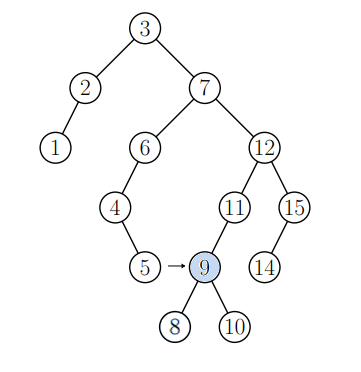
\includegraphics[width = 0.4\linewidth]{figs/fig1.png}
    \caption{Árvore splay.}
    \label{fig:prob1}
\end{figure}

\paragraph{Resposta 1.}
\begin{figure}[h]
    \centering
    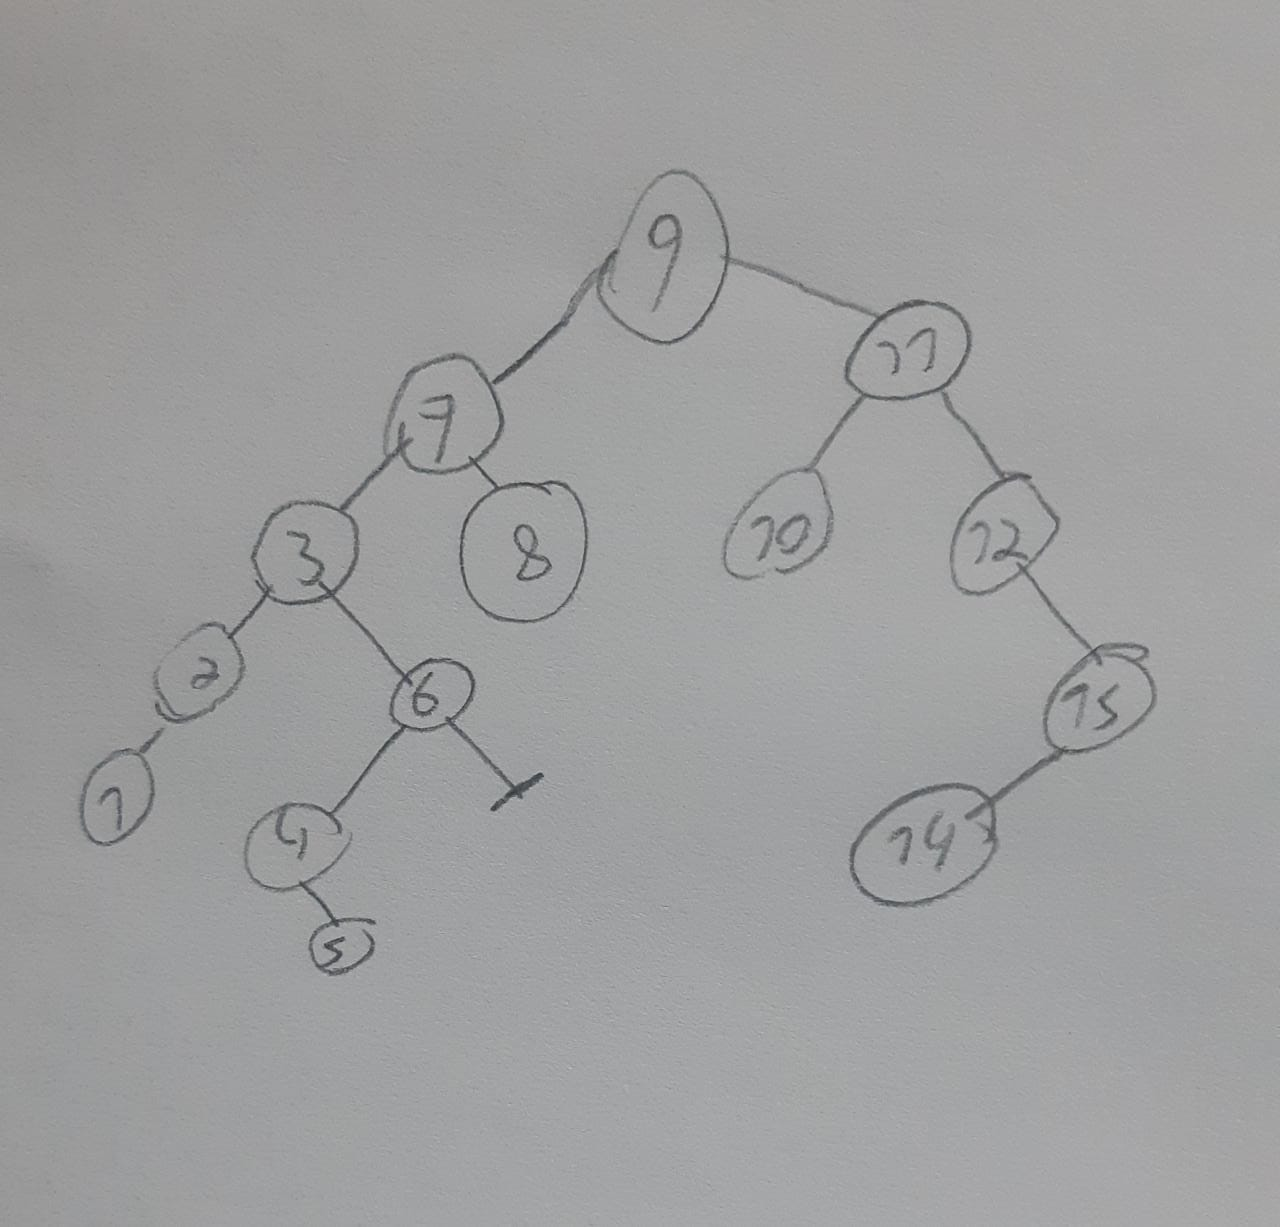
\includegraphics[width = 0.4\linewidth]{figs/fig3.png}
    \caption{resposta 1}
    \label{fig:prob1}
\end{figure}

\paragraph{Problema 2.} (20 pontos)
É fácil ver que, se você usar \textit{splay} duas vezes na mesma \textit{key} em uma \textit{splay-tree} (\texttt{splay(x); splay(x)}), a estrutura da árvore não muda na segunda chamada.
%
Isso é verdade quando alternamos entre duas \textit{keys}? Seja $T_0$ uma \textit{splay tree} e sejam $x$ e $y$ sejam \textit{keys} dentro de $T_0$. Seja:

\begin{itemize}
    \item $T_1$ o resultado de aplicar \texttt{splay(x); splay(y)} em $T_0$.
    \item $T_2$ o resultado de aplicar \texttt{splay(x); splay(y); splay(x); splay(y)} em $T_0$.
\end{itemize}

Independentemente da árvore inicial $T_0$ e da escolha de $x$ e $y$, vale que $T_1 = T_2$? (Que
é, as duas árvores são estruturalmente idênticas?) Ou declare isso como um teorema e prove ou
forneça um contra-exemplo, fornecendo a árvore $T_0$ e duas chaves $x$ e $y$ para as quais isso falha.

\paragraph{Resposta 2.} dando splay(x), x será a raiz, mas dando splay (y), y será a raiz, como as raizes são diferentes, as árvores são diferentes;

\paragraph{Problema 3.} (27 pontos) 
Para este problema, suponha que a estrutura de um nó em
uma \textit{skip list} é a seguinte:

\begin{lstlisting}
class SkipNode {
    Key key; // chave
    Value value; // valor
    vector<SkipNode> next; // vector de pointeiros proximos
}
\end{lstlisting}

A altura de um nó (ou seja, o número de níveis para os quais ele contribui) é dada pela \textit{p.next.size()}.
Muitas vezes, ao lidar com dicionários ordenados, desejamos realizar uma sequência de buscas em ordem. Suponha que temos duas chaves, $x < y$, e já encontramos o nó $p$ que contém a chave $x$. Para encontrar $y$, seria um desperdício coemçar a busca no início do \textit{skip list}. Em vez disso, queremos começar em $p$. Suponha que existam $k$ nós entre
$x$ e $y$ na \textit{skip list}. Queremos que o tempo de busca esperado seja $O(\log k)$, não $O(\log n)$.

\begin{itemize}
    \item (a) Apresentar pseudocódigo para um algoritmo para uma função \texttt{Value ForwardSearch(p, y)}, que iniciando em um nó $p$ (cuja chave é menor que $y$), encontra o nó da \textit{skip list} que contém chave $y$ e retorna seu valor. (Para simplificar, você pode assumir que a chave $y$ aparece dentro da \textit{skip list}.) Além do pseudocódigo, explique brevemente como seu método funciona.
    \item (b) Vamos provar que o valor espeardo de saltos feitos pelo seu algoritmo é $O(\log k)$, onde $k$ é o
número de nós entre $x$ e $y$. Primeiro prove que o nível máximo alcançado esperado é $O(\log k$).
    \item (c) Prove que o número de saltos (\textit{hops}) por nível esperado é $O(1)$.
\end{itemize}

\paragraph{Resposta 3.}

\paragraph{Problema 4.} (20 pontos)
Suponha que você receba uma estrutura de dados \textit{treap} armazenando $n$ chaves. A estrutura do nó
é mostrado na Fig.~\ref{fig:prob4}. Você pode supor que todas as chaves e todas as prioridades são distintas.

\begin{figure}[h]
    \centering
    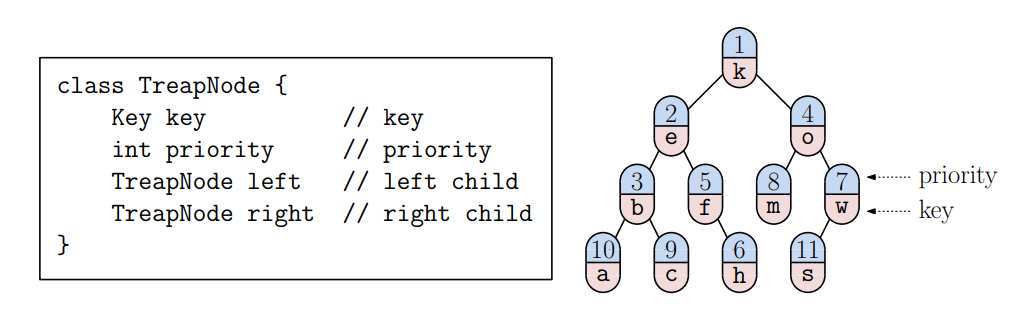
\includegraphics[width = 0.8\linewidth]{figs/fig2.png}
    \caption{Estrutura do nó da \textit{treap} e exemplo.}
    \label{fig:prob4}
\end{figure}

\begin{itemize}
    \item (a) Apresente um pseudocódigo para a função \texttt{int minPriority(Key x0, Key x1)}, que é dado duas chaves $x_0$ e $x_1$ (que podem ou não estar na \textit{treap}), e retorna o
prioridade mais baixa entre todos os nós cujas chaves $x$ estão no intervalo $x_0 \leq x \leq x_1$. Se a \textit{treap}
não tem chaves neste intervalo, a função retorna \texttt{int MAXVAL}. Explique brevemente por que
sua função está correta. Por exemplo, na Fig.~\ref{fig:prob4} a chamada \texttt{minPriority("c", "g")} retornaria $2$ do nó
\texttt{"e"}, pois é a prioridade mais baixa entre todas as chaves $x$ onde $"c" \leq x \leq "g"$.
\item (b) Assumindo que a treap armazena $n$ chaves e tem altura $O(\log n)$, qual é o tempo de execução
do seu algoritmo? (Justifique brevemente sua resposta.)
\end{itemize}

\paragraph{Resposta 4.}

\paragraph{Problema 5.} (23 pontos)
Defina uma nova operação de \textit{treap}, \texttt{expose(Key x)}. Ele encontra a chave $x$ na árvore (jogando
uma exceção se não for encontrada), define sua prioridade para $-\infty$ (ou mais praticamente \texttt{int MAXVAL}),
e, em seguida, restaura a ordem de prioridade da \textit{treap} por meio de rotações. (Observe que o nó contendo $x$ será rotacionado para a raiz da árvore.) Apresente o pseudocódigo para esta operação.

\paragraph{Resposta 5.}

\section{Detalhes avaliação}
Uma pergunta comum é "quanto detalhe é esperado nas respostas?", algumas orientações são:
%
\paragraph{Provar vs. Mostrar:}
Se lhe pedirmos para “provar” algo, estamos à procura de uma prova bem estruturada. Se você estiver aplicando a indução, tenha cuidado para distinguir seu(s) caso(s) básico(s) e indicar qual é a sua hipótese de indução. Se lhe pedirmos para “mostrar”, “explicar” ou “justificar”, estaremos geralmente apenas esperando uma explicação em português. Se você não tiver certeza, por favor, verifique.

\paragraph{Algoritmo vs. Pseudocódigo:} Quando pedimos um “algoritmo” estamos esperando uma descrição em alto nível de algum processo computacional, geralmente em uma combinação de português e notação matemática (por exemplo, “classifique as $n$ chaves e localize $x$ usando busca binária”). Para pseudocódigo, nós estão esperando uma descrição passo a passo mais detalhada que se pareça muito mais com C++ (por exemplo, “\texttt{Node q = p.left}”). Lembre-se de que você está escrevendo seu código para ser lido por um humano, e não por um compilador. Por favor, omita detalhes irrelevantes que são sintaxes de C++. Mesmo que não solicitemos explicitamente, sempre que você fornecer um algoritmo ou pseudocódigo, você deve sempre fornecer uma breve explicação em português. Isso ajuda o avaliador a entender quais são suas intenções, e se houver um pequeno erro em seu código, muitas vezes podemos usar seu explicação para entender quais eram suas reais intenções.

\end{document}


